% !TEX root = sum1.tex

\section{Results}
% The nested structure makes the greedy method useful.
% Remark: Similar to what we mentioned, the greedy method refers to using the largest groups to fill the seats.


% Improvement:
% For $\X^{0}$, we introduce one empty seat, $x_1$. But it cannot provide the feasibility.

% \subsection{Deterministic Model}\label{Deterministic_result}
% The integer programming \eqref{deter_upper} can be solved quickly because of the monotone ratio.


\subsection{Benders Decomposition versus IP}\label{Bender_IP}

% In view of the fact that IP of the deterministic model can be solved quickly, the column generation method does not show an obvious advantage. 

% At first, we compare the running time of these two methods. 

The running times of solving IP directly and using Benders decomposition are shown in Table \ref{tab_1}. 

\begin{table}[ht]
  \centering
  \caption{Running time of Decomposion and IP}\label{tab_1}
  \begin{tabular}{|l|l|l|l|l|l|l|}
  \hline
  \# of scenarios & demands & running time of IP(s) & Benders (s) & \# of rows & \# of groups & \# of seats\\
  \hline
  1000  & (150, 350) & 5.1  & 0.13 & 30 & 8 & (21, 50)\\
  5000  & & 28.73 & 0.47 & 30 & 8 \\
  10000 & & 66.81  & 0.91 & 30 & 8 \\
  50000 & & 925.17 & 4.3 & 30 & 8 \\
  \hline
  1000  & (1000, 2000) & 5.88 & 0.29 & 200 & 8 & (21, 50)\\
  5000  & & 30.0 & 0.62 & 200 & 8 \\
  10000 & & 64.41 & 1.09 & 200 & 8 \\
  50000 & & 365.57 & 4.56 & 200 & 8 \\
  \hline
  1000  & (150, 250) & 17.15  & 0.18 & 30 & 16 & (41, 60) \\
  5000  & & 105.2  & 0.67 & 30 & 16  \\
  10000 & & 260.88 & 1.28 & 30 & 16  \\
  50000 & & 3873.16 & 6.18 & 30 & 16  \\
  \hline
  \end{tabular}
\end{table}

The parameters in the columns of the table are the number of scenarios, the range of demands, running time of integer programming, running time of Benders decomposition method, the number of rows, the number of group types and the number of seats for each row, respectively. 

Take the first experiment as an example, the scenarios of demands are generated from (150, 350) randomly, the number of seats for each row is generated from (21, 50) randomly.
% about 1000 seats.

% The second one:
% The number of seats for each row L is generated from (21, 50) randomly, about 7000 seats.
% The scenarios of demands are generated from (1000, 2000) randomly.

% The third one:
% The number of seats for each row L is generated from 41-60 randomly, about 1500 seats.
% The scenarios of demands are generated from (150, 250) randomly.


\subsection{Near-optimal Solution versus IP Solution under Nested Policy}
Then, we will show the near-optimal seat assignment has a close performance with IP when considering nested policy.

% Then we compare the results of benders decomposition and IP under nested policy.

\begin{table}[ht]
    \caption{Results of Decomposion and IP under nested policy}
    \begin{tabular}{|l|l|l|l|l|l|}
    \hline
    \# samples & T & probabilities & \# rows & people served by decomposition & people served by IP \\
    1000  & 45  & [0.4,0.4,0.1,0.1] & 8 & 85.30 & 85.3 \\
    1000  & 50  & [0.4,0.4,0.1,0.1] & 8 & 97.32 & 97.32 \\
    1000  & 55  & [0.4,0.4,0.1,0.1] & 8 & 102.40 & 102.40  \\ % slow
    1000  & 60  & [0.4,0.4,0.1,0.1] & 8 & 106.70 & NA  \\
    1000  & 65  & [0.4,0.4,0.1,0.1] & 8 & 108.84 & 108.84 \\
    \hline
    1000  & 35  & [0.25,0.25,0.25,0.25] & 8 & 87.16 & 87.08 \\
    1000  & 40  & [0.25,0.25,0.25,0.25] & 8 & 101.32 & 101.24 \\
    1000  & 45  & [0.25,0.25,0.25,0.25] & 8 & 110.62 & 110.52 \\
    1000  & 50  & [0.25,0.25,0.25,0.25] & 8 & 115.46 & NA \\
    1000  & 55  & [0.25,0.25,0.25,0.25] & 8 & 117.06 & 117.26 \\
    \hline
    5000  & 300  & [0.25,0.25,0.25,0.25] & 30 & 749.76 & 749.76 \\
    5000  & 350  & [0.25,0.25,0.25,0.25] & 30 & 866.02 & 866.42 \\
    5000  & 400  & [0.25,0.25,0.25,0.25] & 30 & 889.02 & 889.44 \\
    5000  & 450  & [0.25,0.25,0.25,0.25] & 30 & 916.16 & 916.66 \\
    \hline
    \end{tabular}
\end{table}

Each entry of people served is the average of 50 instances.
IP will spend more than 2 hours in some instances, as `NA' showed in the table.
The number of seats is 20 when the number of rows is 8, the number of seats is 40 when the number of rows is 30.

We can find that the people served by Benders decomposition and IP under nested policy are close. But obtaining the near-optimal seat assignment will be faster.

% Thus, we can use the near-optimal seat assignment from the decomposition approach.

\subsection{Different Probabilities}
We discuss the effect of different probabilities in this sub-section. Suppose that the group of up to 4 can sit together. Then we have $E(D) = (p_1 * 1 + p_2 * 2 + p_3 * 3 + p_4 * 4) T$. Let $c = p_1 * 1 + p_2 * 2 + p_3 * 3 + p_4 * 4$. Choose $T(E(D)/c)$ such that the supply is near the demand. Then we compare the number of people served under different values of $c$. 

% by FCFS-based.

% Different $T$ has little effect on the number of people served using M6 because it is based on first-come-first-served. 


Sample $p_1, p_2, p_3$ from $0.05$ to $0.95$ with increment of $0.5$. The number of rows is 10, and the number of seats for each row is 21 (including one dummy seat). The number of periods is $200$. The number of people served with respect to the value of $c$ is shown below:

% \begin{figure}[h]
%   \centering
%   \subfigure[One instance for each data point]{
%     \label{Fig.sub.1}
%     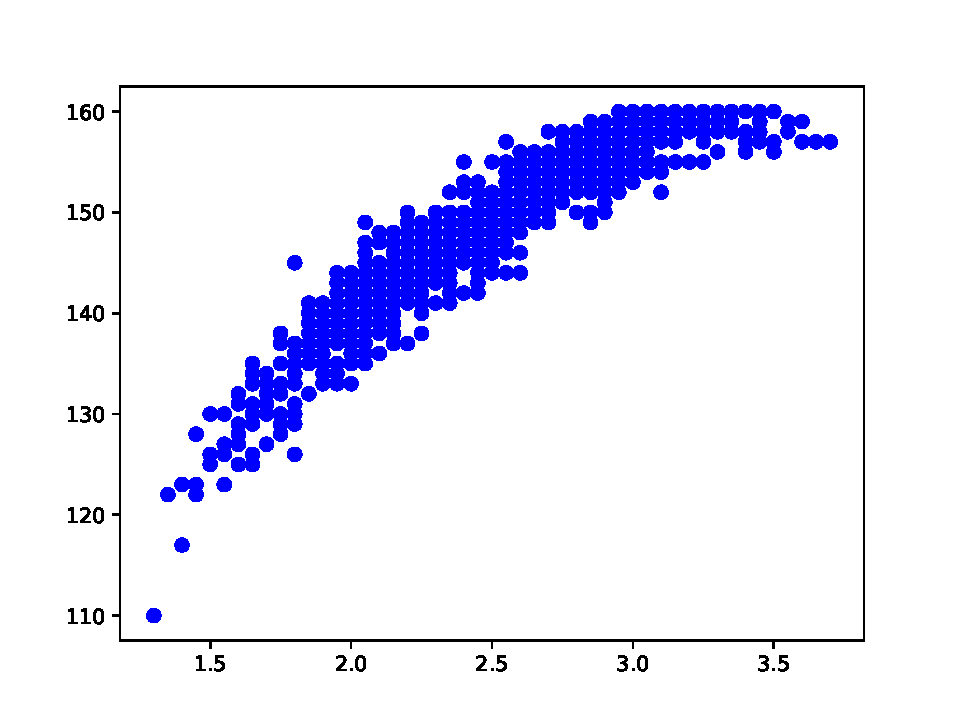
\includegraphics[width=0.48\textwidth]{./Figures/Figure_1.pdf}}
%   \subfigure[Average of 50 instances for each data point]{
%     \label{Fig.sub.2}
%     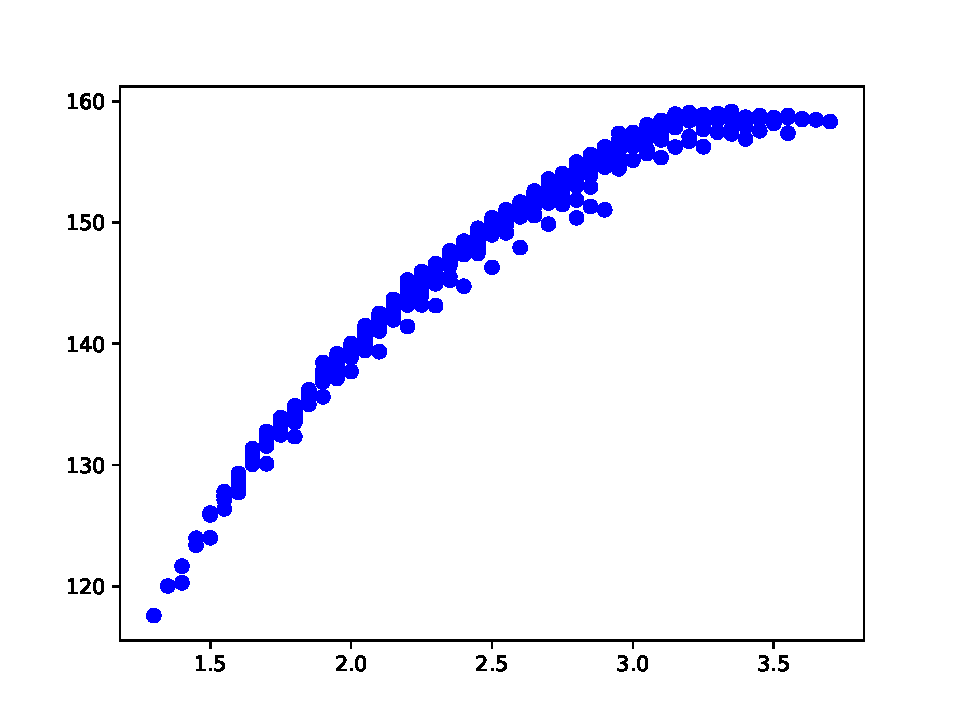
\includegraphics[width=0.48\textwidth]{./Figures/Figure_2.pdf}}
%   \caption{The number of people served versus $c$}
%   \label{Fig.lable}
% \end{figure}

\begin{figure}[ht]
  \centering
  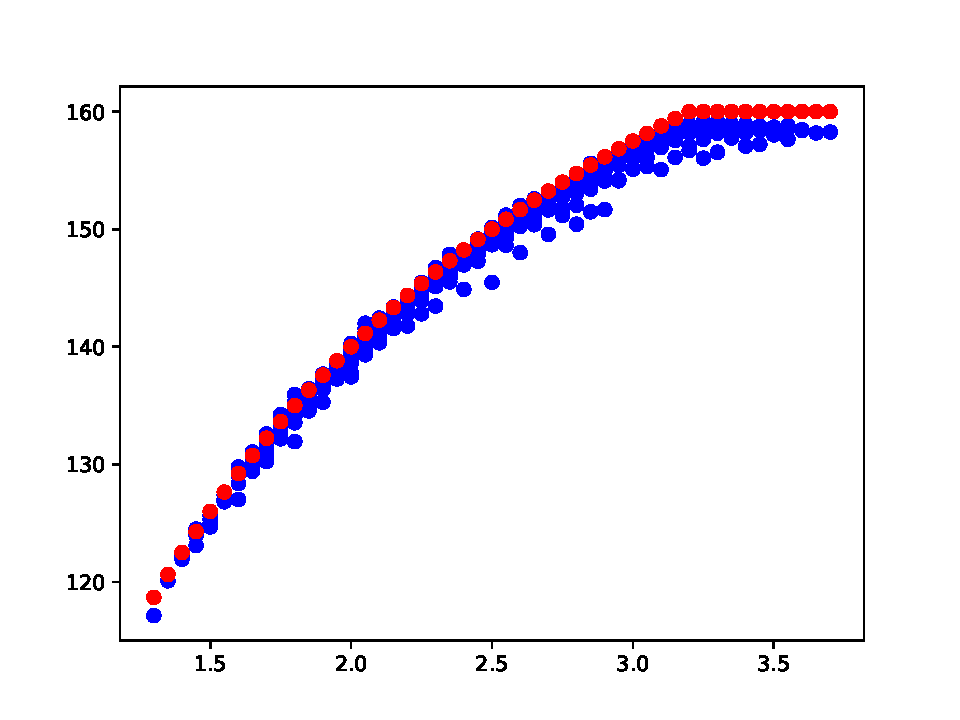
\includegraphics[width = 0.7\textwidth]{./Figures/diff_2.pdf}
  \caption{The number of people served versus $c$}
\end{figure}

Each blue point stands for the average number of people of 50 instances.
Each red point stands for the expected number of people.

Suppose we accept $D_a$ people with $T$ arrivals and the sum of $D_a$ and $T$ is equal to the total number of seats.($D_a = c * T$) Then the estimation of occupancy rate is $\frac{c * T}{(c+1) * T}= \frac{c}{c+1}$ when there are full patterns for all rows.


The number of people served is near $\frac{c}{c+1} * 210$ on average.(Red points showed in the figure.) 

If the largest pattern is assigned for each row, then the occupancy rate is $\frac{16}{21}$. The maximal number of people can be served is $210 * \frac{16}{21} =160$ which is the upper bound of the number of people served.

From the above figure, we can also find that some blue points are far from the red points. For example, when the probability is $[0.05, 0.05, 0.85, 0.05](c =2.9)$, the demands can be $[4, 1, 45, 2]$ or $[2, 2, 47, 1]$. We cannot construct all full patterns for every row with these demands. It violates the assumption, thus in this case there is a large gap between blue point and red point.


% When $p = [0.25, 0.25, 0.25, 0.25]$, $E(D) = 2.5 T$. Let $p_1*1 + p_2*2 + p_3*3 + p_4*4 = 2.5$, 
% Let $E(D) = 150, T = 50, 60, 75$. The number of seats: 200, 210, 225.

% 1: When $E(D)$ is fixed, case3,4 need a larger hall to accept the same number of people.

% Different layout may make a difference.

% 2. The assumption that $T$ is fixed will be more reasonable for the continuous time. 

\newpage

Let $E(D) = 150$.

Two experiments:
When $E(D) = 2.5T$, which means on average 2.5 people arrive for each group.

$T =75$, the number of rows is 9, the number of seats each row is 25.

Probabilities: 
$p_1 = p_3 + 2p_4$. $p_3$ is from $0.05$ to $0.45$ with step size of 0.1. $p_4$ is from $0.05$ to $0.3$ with step size of 0.05.

% Results: M1-M6, the number of accepted people, the number of total people.

% 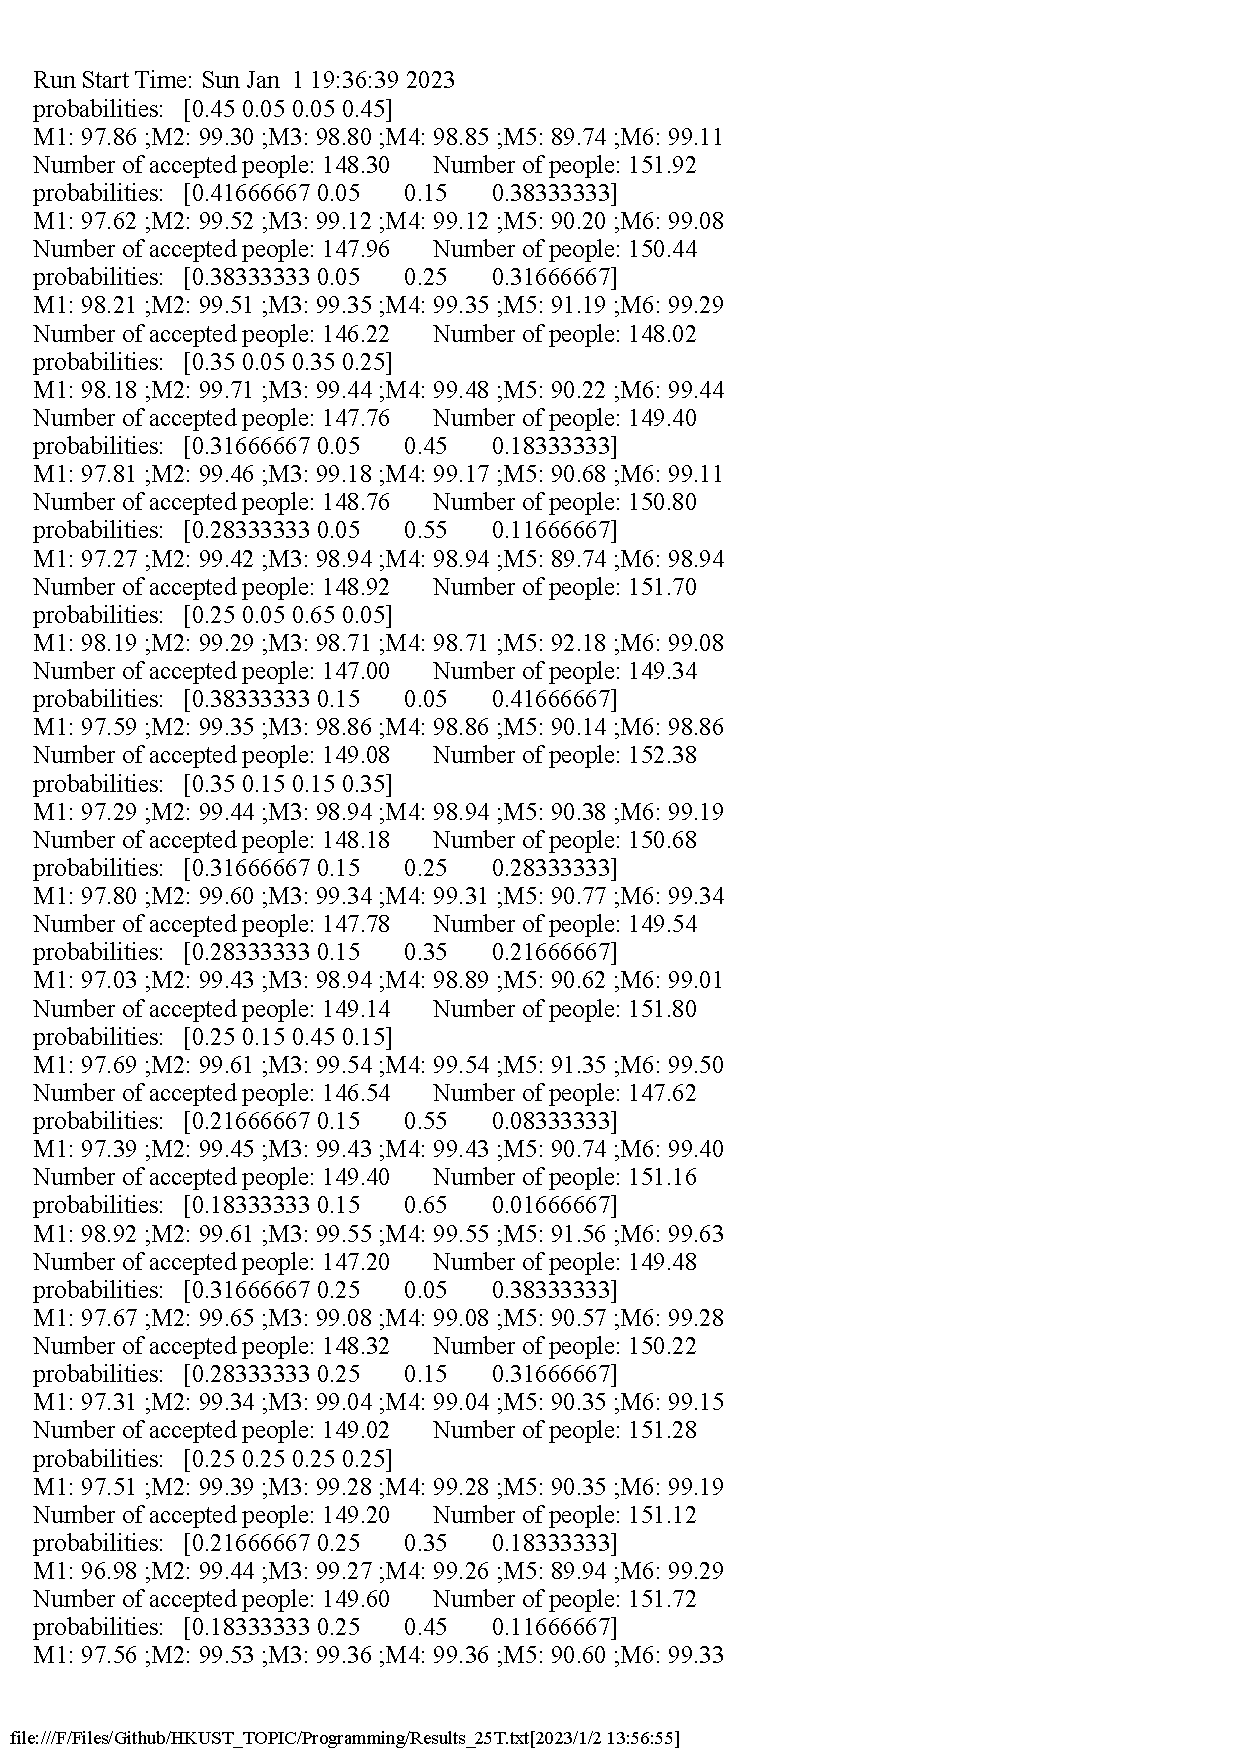
\includepdf{./Figures/Results_25T.pdf}

When $E(D) = 2T$, which means on average 2 people arrive for each group.

$T = 60$, the number of rows is 10, the number of seats each row is 21.

Probabilities: 
$2p_2 + 4p_3 + 6p_4 =3$. $p_2$ is from $0.05$ to $0.95$ with step size of $0.1$. $p_3$ is from $0.05$ to $0.75$ with step size of $0.1$.

% Results: M1-M6, the number of accepted people, the number of total people.

% 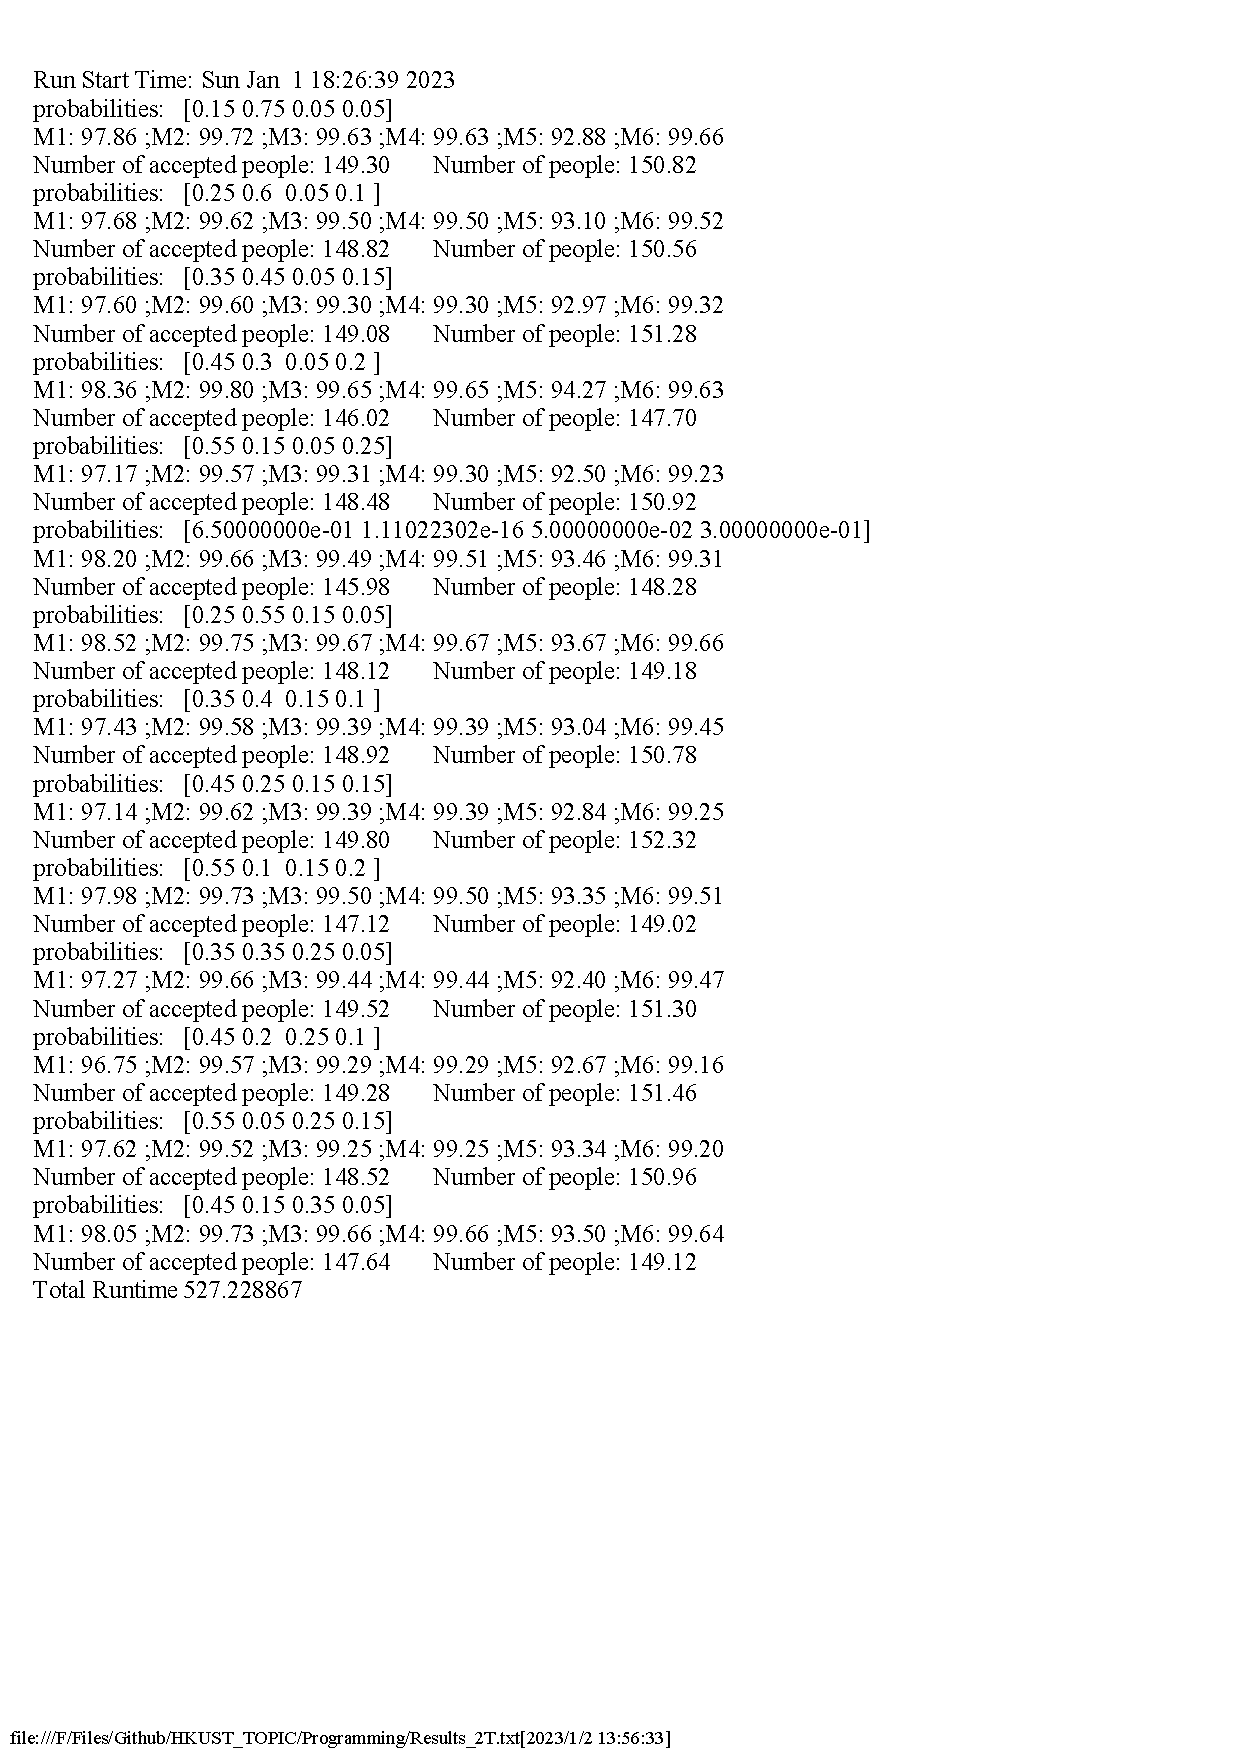
\includepdf{./Figures/Results_2T.pdf}

\subsection{Different Periods}
We discuss the effect of the number of periods this sub-section. 

Parameters: T = 10-100, step size =1.

The expected number of period: 60
The expected number of demand(people): 150
Number of rows: 10
Number of seats each row: 21
Probabilities: $[0.25, 0.25, 0.25, 0.25]$.

Parameters: T = 30-120, step size =1.

The expected number of period: 72
The expected number of demand(people): 137
Number of rows: 10
Number of seats each row: 21
Probabilities: $[0.4, 0.4, 0.1, 0.1]$

% [0.3, 0.5, 0.1, 0.1]$.
% Results: M1-M6, the number of accepted people, the number of total people.

% 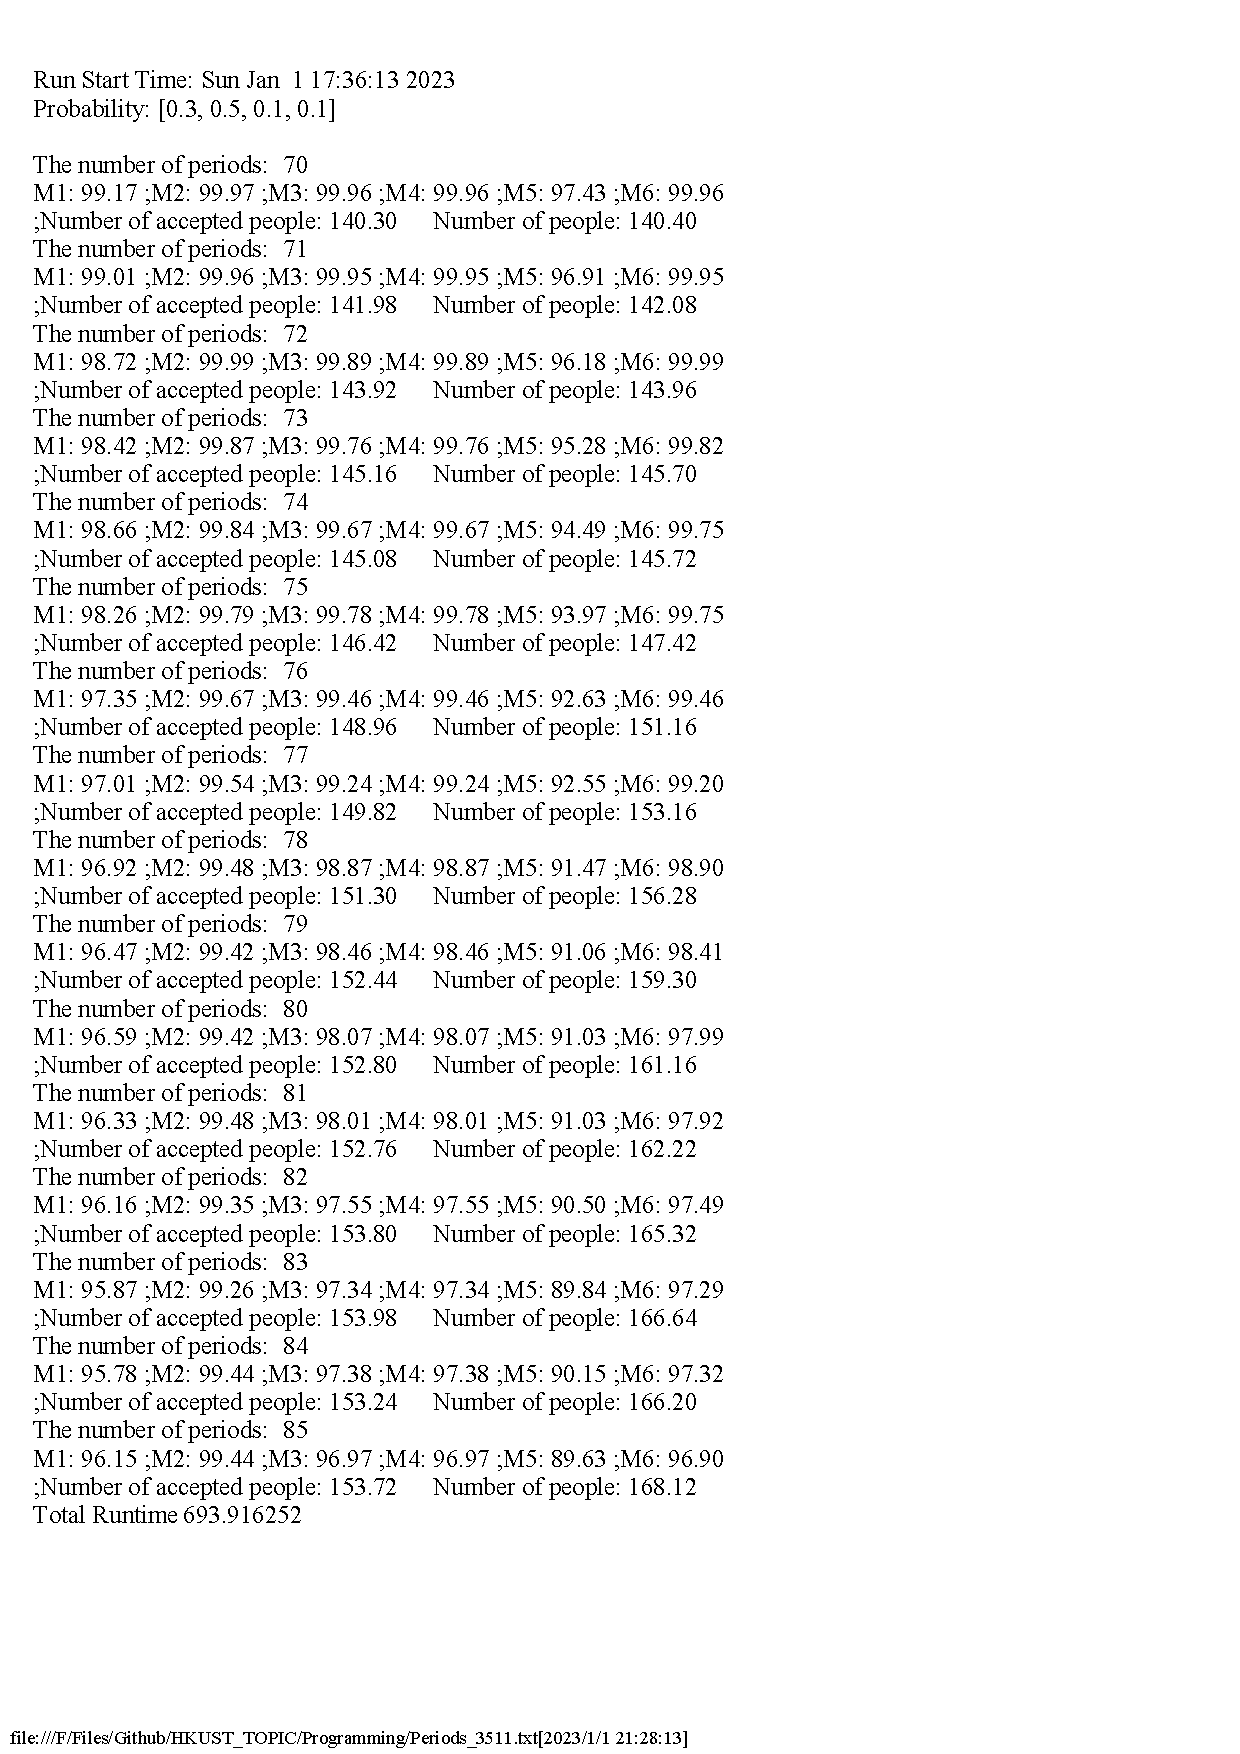
\includepdf{./Figures/Periods_3511.pdf}
% 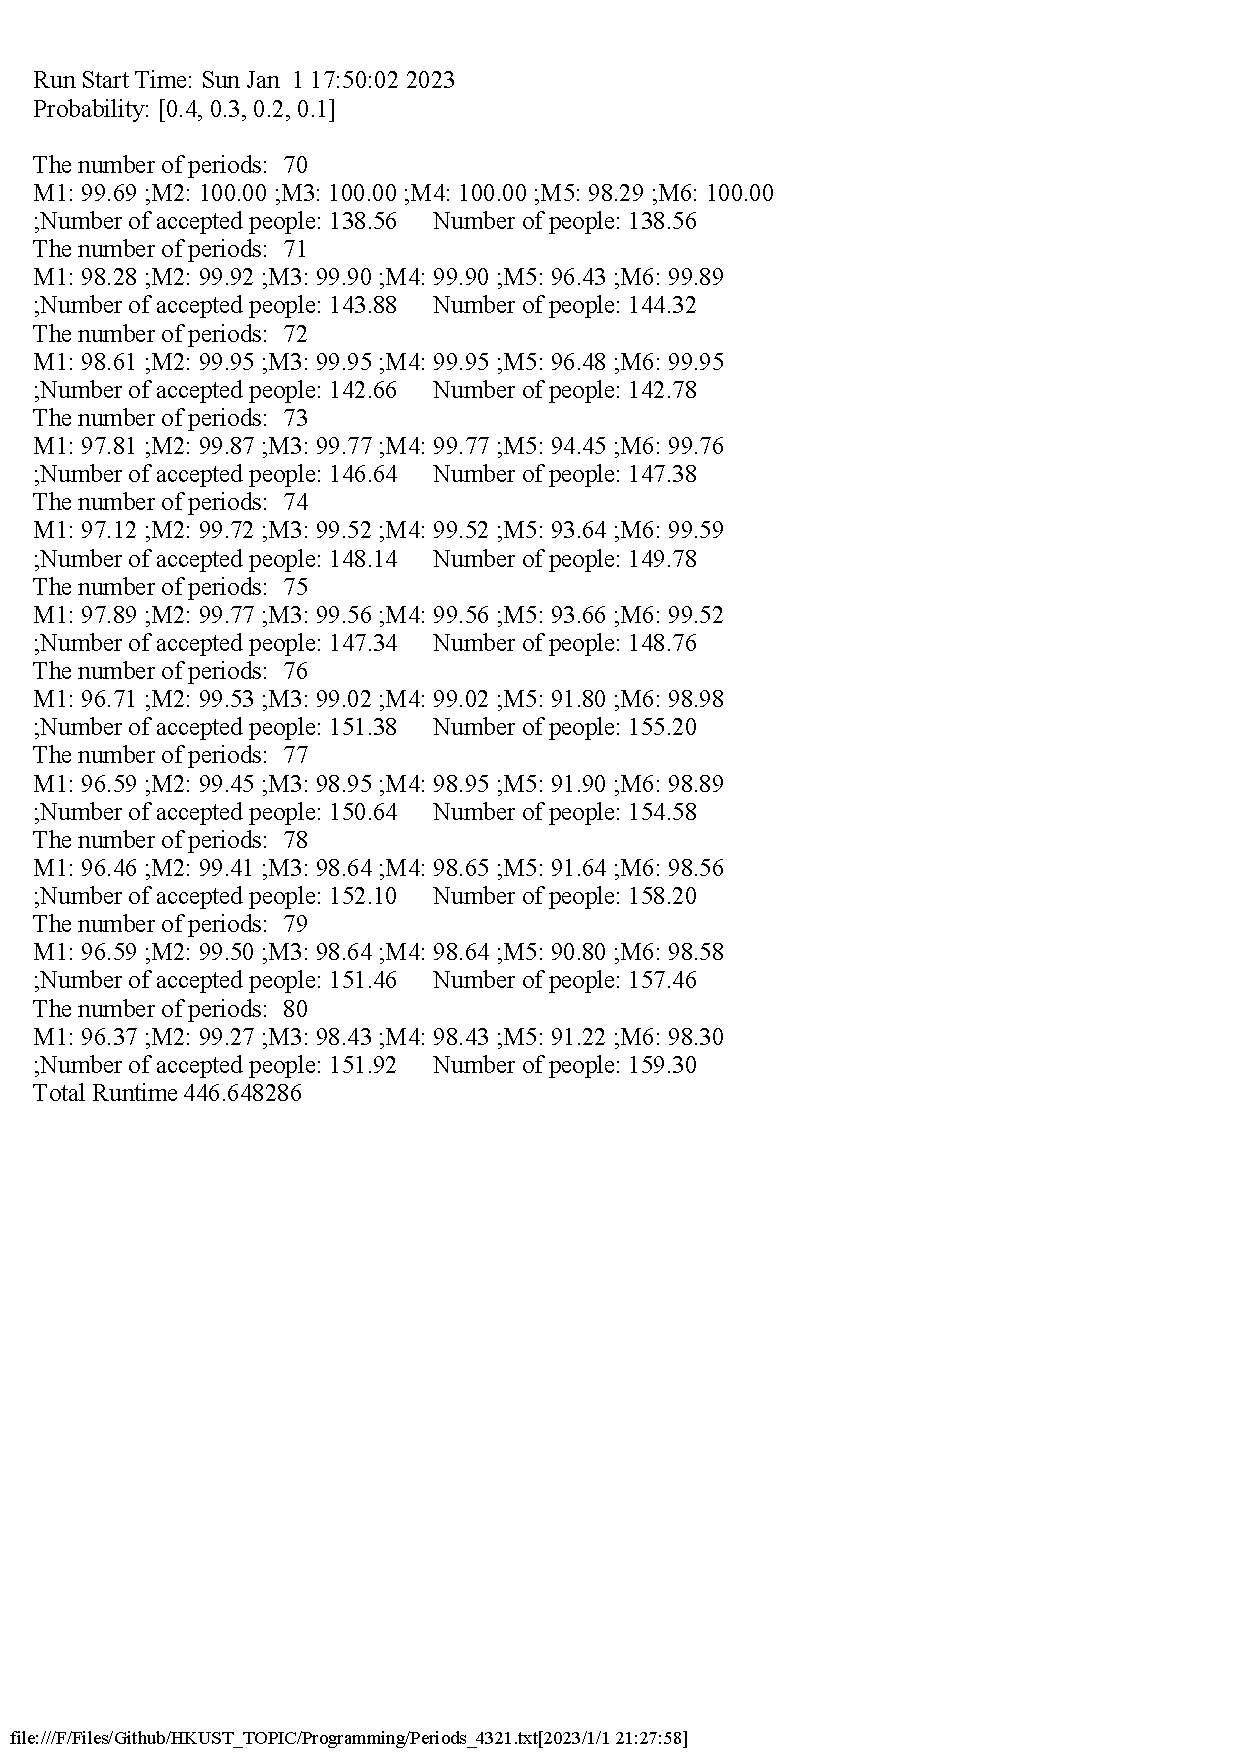
\includepdf{./Figures/Periods_4321.pdf}


% Results: M1-M6, the number of accepted people, the number of total people.

We can find that the difference between the number of accepted people and the number of total people will increase with the period. 
% When the number of periods is small, the seats 

Probability 1: $[0.25, 0.25, 0.25, 0.25]$,
Probability 2: $[0.4, 0.4, 0.1, 0.1]$

\begin{figure}[h]
  \centering
  \subfigure[Probability 1]{
    \label{Fig.sub.1}
    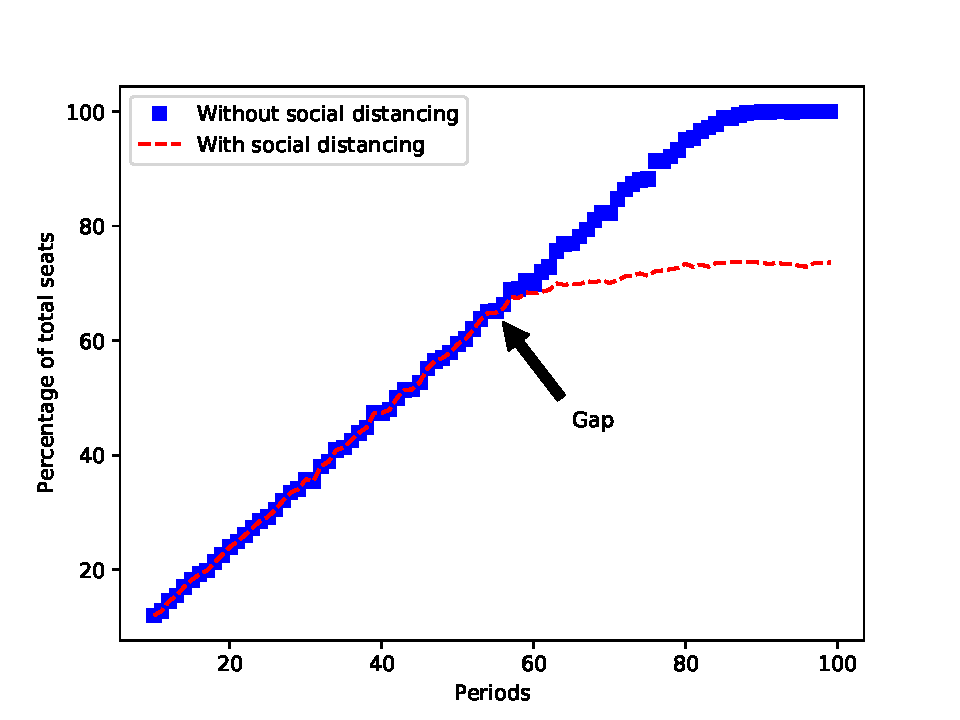
\includegraphics[width=0.48\textwidth]{./Figures/period_1.pdf}}
  \subfigure[Probability 2]{
    \label{Fig.sub.2}
    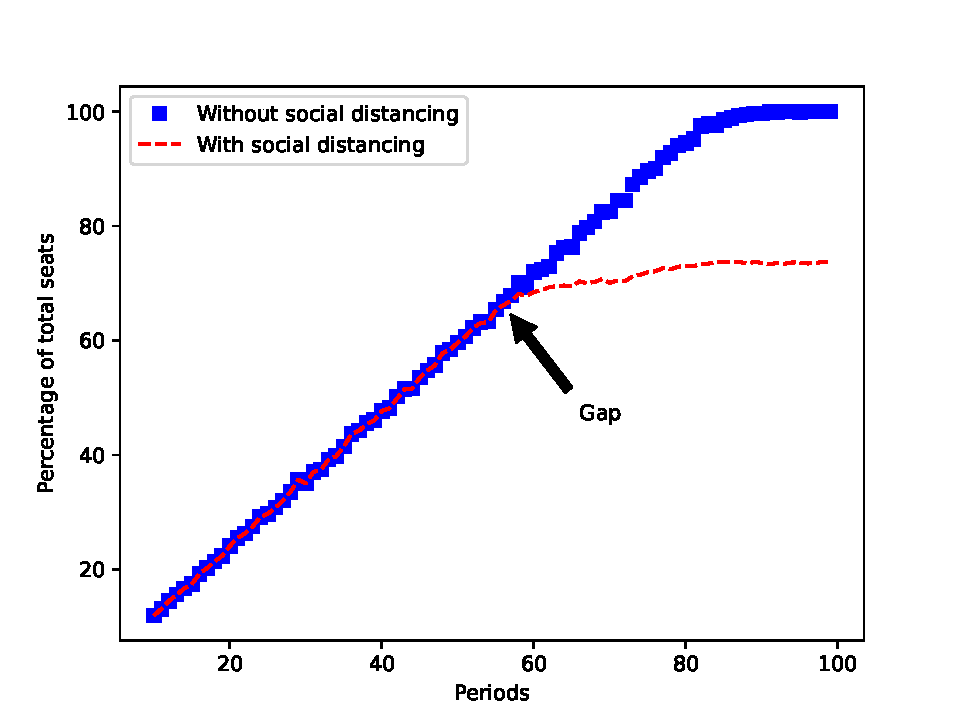
\includegraphics[width=0.48\textwidth]{./Figures/period_2.pdf}}
  \caption{The number of people served versus periods}
  \label{Fig.lable}
\end{figure}

There are three stages, 

First stage: the capacity is sufficient. The social distancing will not cause any effect.

Second stage: the gap is becoming larger as $T$ increases. 

Third stage: As $T$ continues to increase, the gap will converge when the capacity is limited.

The gap point represents the first point where the people without social distancing is larger than that with social distancing. 

The government can make the policy about how much attendance rate.

\subsection{Group of Different Sizes}

% \subsection{Measurement}

% Suppose a real scenario with a fixed sequence, $s^{r}$. Solving the following program can obtain the optimal value, $V_{s^{r}}$. (Offline)

% Then the difference is $V_{s^{r}} - \text{our result}$.

% WS(the value under wait-and-see policy with all possible scenarios)

% EVPI(Expected Value of Perfect Information) = WS - the value of deterministic equivalent form

% Regret.

% Several things need to do:

% What is greedy result like?

% Why does period run so slowly?

% Revise lemma

% lack of the traits


\newpage
